\newpage
\section{Anwendung}
Die Anwendung zur Steuerung der Applikation, welche mit Unity entwickelt wurde, bietet diverse Möglichkeiten zur Darstellung,
das Umschalten von Spielmodi und das Erzeugen eines Spielstands zwecks Debugging/Testing.
Die Funktionalitäten werden nachfolgend beschrieben.

\begin{minipage}[t]{0.2\textwidth}
    \begin{center}
        
\includegraphics[width=0.3\linewidth]{../common/03_billiard_ai/resources/41_halo.png}
    \end{center}
\end{minipage}\hfill
\begin{minipage}[t]{0.8\textwidth}
    \textbf{Halo}: Der Halo um die Kugel kann über die Taste \textbf{H} angezeigt oder versteckt werden.
\end{minipage}\vskip.2\baselineskip
\textbf{Löcher und Banden}: Die Löcher und Banden können über die Taste \textbf{T} angezeigt oder versteckt werden, siehe Abbildung \ref{fig:display_table_rail_targets}.
\begin{figure}[h!]
    \begin{center}
        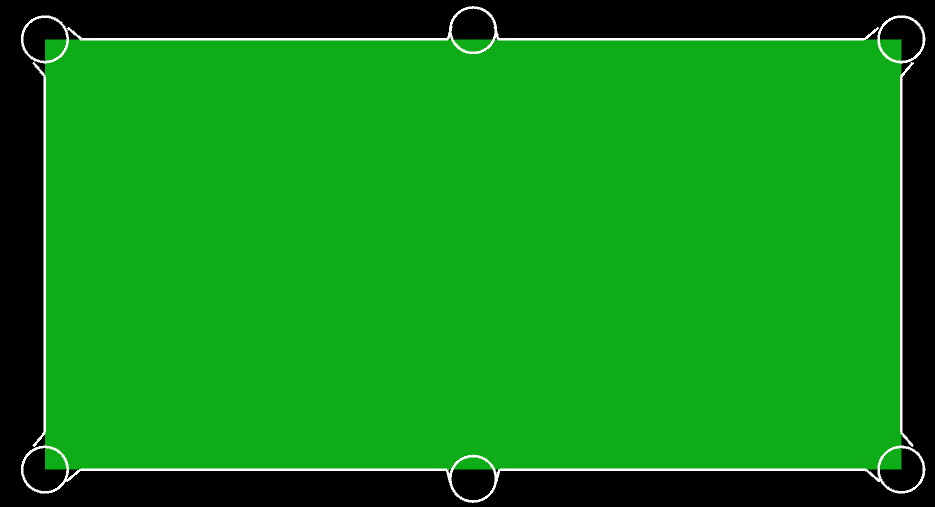
\includegraphics[width=0.4\linewidth]{../common/03_billiard_ai/resources/42_empty_table_with_rails_and_pockets.png}
    \end{center}
    \caption{Anzeige des Tisches mit Banden und Löchern}
    \label{fig:display_table_rail_targets}
\end{figure}\\
\begin{minipage}[t]{0.2\textwidth}
    \begin{center}
        
\includegraphics[width=0.3\linewidth]{../common/03_billiard_ai/resources/43_ball_dot.png}
    \end{center}
\end{minipage}\hfill
\begin{minipage}[t]{0.8\textwidth}
    \textbf{Punktpfad}: Über die Taste \textbf{P} kann ein Pfad bestehend aus Punkten eingeblendet werden. Diese Punkte
    werden jeweils an einer Kugelposition für zwei Sekunden angezeigt. Dies ermöglicht die visuelle Pfadverfolgung einer
    Kugel.
\end{minipage}\vskip.2\baselineskip
\textbf{Livemode}: Die Livedetektion kann über die Taste \textbf{L} ein- oder ausgeschaltet werden.\\
\textbf{Alle Suchergebnisse anzeigen}: Über die Taste \textbf{X} werden alle Suchergebnisse nacheinander visualisiert. \\
\textbf{Weitere Kugelverläufe ein/ausblenden}: Über die Taste \textbf{Q} kann die Anzeige über gestrichelte Linien der weiteren
Kugelverläufe ein- und ausgeblendet werden.\\
\textbf{Infinity-Mode}: Über die Taste \textbf{M} kann der Infinity-Modus ein- oder ausgeschaltet werden.
Dieser ist standardmässig deaktiviert. Im Infinity-Modus werden gewisse Regeln des Spiels ignoriert. Es wird erkannt,
wann der Spielstand stabil bleibt, sich demnach nichts bewegt. In diesem Fall wird automatisch eine Suche ausgelöst
und das Resultat angezeigt. Dieser Modus hat die Intention aufzuzeigen, wie man eine Kugel anspielen muss und soll
möglichst wenig direkte Interaktion mit dem Computersystem erfordern.\\
\textbf{Tiefensuche}: Die Suche über mehrere Stösse kann über die Taste \textbf{Y} ein- und ausgeschaltet werden.\\
\textbf{Mehrere Geschwindigkeiten}: Die Suche mit mehreren Geschwindigkeiten kann über die Taste \textbf{V} ein- und ausgeschaltet werden.\\
\textbf{Animationsfunktionalitäten}: Die Animation eines Stosses wird automatisch nach der Suche
ausgelöst. Eine pausierte Animation ist in Abbildung \ref{fig:unity_animation} ersichtlich.
Mittels der Tasten \textbf{Pfeil links} und \textbf{Pfeil rechts} kann innerhalb des Stosses nach vorne oder zurück
gespult werden. Mit den Tasten \textbf{Pfeil oben} und \textbf{Pfeil unten} kann zwischen verschiedenen Stössen gewechselt
werden. Es kann gut sein, dass der erste Stoss jeweils derselbe ist, Unterschiede können erst in tieferen Stössen auftreten.
Mit der \textbf{Leertaste} kann eine Animation gestoppt und mit der \textbf{Return-Taste} auf Anfang zurückgesetzt werden.
\begin{figure}[h!]
    \begin{center}
        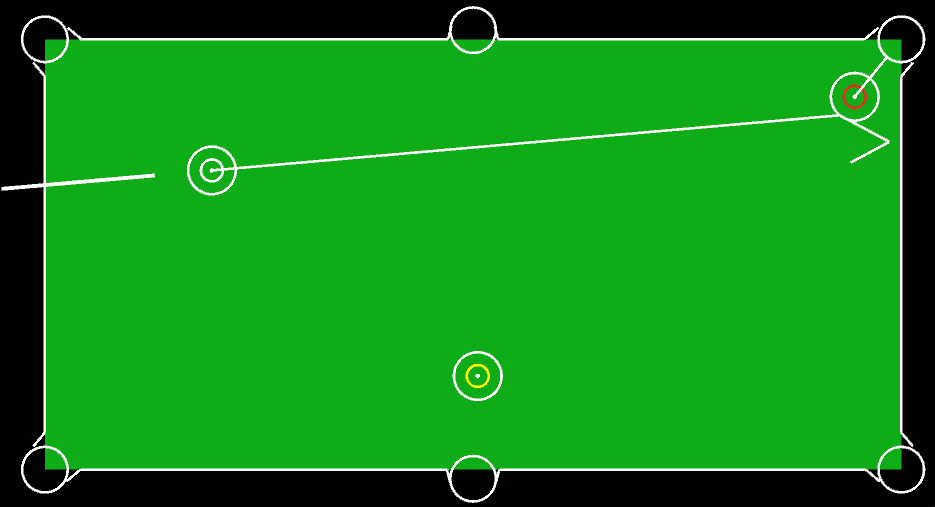
\includegraphics[width=0.4\linewidth]{../common/03_billiard_ai/resources/44_animation.png}
    \end{center}
    \caption{Unity Animationsdarstellung}
    \label{fig:unity_animation}
\end{figure}\\
\begin{minipage}[t]{0.2\textwidth}
    \begin{center}
        
\includegraphics[width=0.3\linewidth]{../common/03_billiard_ai/resources/45_unity_yellow_ball.png}
        
\includegraphics[width=0.3\linewidth]{../common/03_billiard_ai/resources/45_unity_yellow_ball_2.png}
    \end{center}
\end{minipage}\hfill
\begin{minipage}[t]{0.8\textwidth}
    \textbf{Anzeige der animierten Kugeln}: Die Kugeln können über die Taste \textbf{K} entweder als Umrandung, volle Kugel
    oder unsichtbar dargestellt werden.
\end{minipage}\vskip.2\baselineskip
\begin{minipage}[t]{0.2\textwidth}
    \begin{center}
        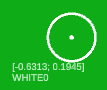
\includegraphics[width=0.3\linewidth]{../common/03_billiard_ai/resources/46_unity_debug_output.png}
    \end{center}
\end{minipage}\hfill
\begin{minipage}[t]{0.8\textwidth}
    \textbf{Informationsausgabe}: Zu Entwicklungszwecken kann die Position und die ID mit der Taste \textbf{D} angezeigt oder versteckt werden.
\end{minipage}\vskip.2\baselineskip
\textbf{Spielstandeingabe}: Ebenfalls zu Entwicklungszwecken kann das Erstellen eines Spielstands über die Taste \textbf{S} erfolgen.
In diesem Modus kann über das Scroll-Rad der Maus der Typ der zu platzierenden Kugel ausgewählt werden. Mit einem linken Mausklick
wird die Kugel platziert, mit einem rechten Mausklick auf eine Kugel wird diese entfernt. Ein Status kann auch textuell beschrieben
eingegeben werden. Dazu kann im Spielstand-Erstellmodus die Taste \textbf{T} gedrückt werden. Es erscheint ein Eingabefeld.
Das Format lautet:
\begin{algorithm}[H]
    ID, TYP, X-Koordinate, Y-Koordinate\\
    ID, TYP, X-Koordinate, Y-Koordinate
\end{algorithm}
Die Erfassung einer weissen und roten Kugel wird nachfolgend beschrieben:\\
\begin{algorithm}[H]
    WHITE0, WHITE, -300, 0\\
    RED1, RED, -150, -300
\end{algorithm}
Sobald die Beschreibung erfasst wurde, kann die Eingabe mit \textbf{Enter} bestätigt werden. Es wird der normale Modus
angezeigt mit dem erstellten Spielstand.